\documentclass[tikz]{standalone}

\usepackage{tikz}

\usetikzlibrary{arrows, automata, topaths, calc, shapes.geometric}

\begin{document}


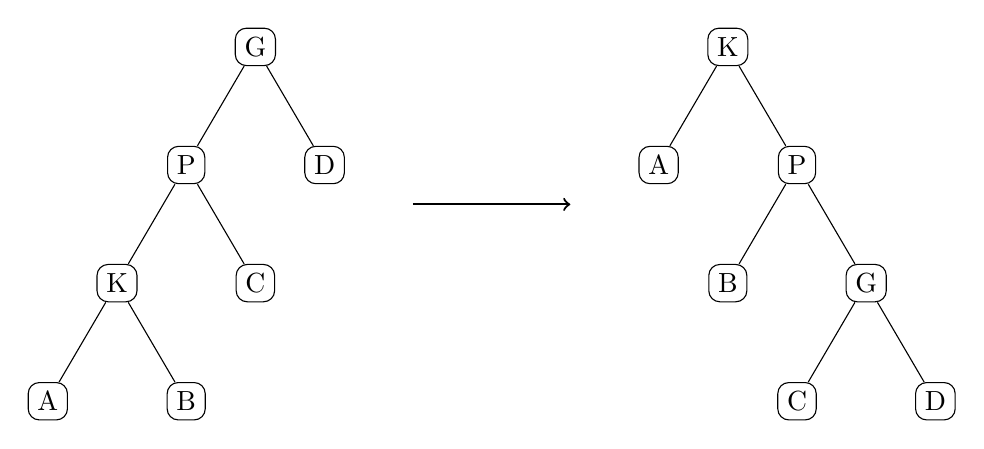
\begin{tikzpicture}[sibling distance=5em,
  every node/.style = {shape=rectangle, rounded corners, draw, align=center}]]

  \node at (2,4) {G} 
    child { node {P} 
      child { node {K} 
         child { node {A} }
         child { node {B} } }
      child { node {C} } }
    child { node {D}};

  \draw[thick, ->] (4,2) -- (6,2);

  \node at (8,4) {K} 
    child { node {A}}
    child { node {P} 
        child { node {B} }
        child { node {G} 
          child { node {C}}
          child { node {D}}}};
\end{tikzpicture}
\end{document}
